\chapter{जनन और पर्यावरण}\label{ch:g8:reproduction-and-environment}

मेंढकों का सामूहिक गान मई में ही क्यों शुरू होता है, नवंबर में क्यों
नहीं? बीच का कोई अच्छा साल जंगल को \omterm{prop:g2:from-seed-to-plant:cycle}{अंकुरों} से क्यों भर देता है, और ठंडी
गीली जून अगले वसंत का तालाब मेंढक के बच्चों से ख़ाली क्यों कर देती है?
पिछले अध्याय ने अगली पीढ़ी की कार्य-प्रणाली बनाई; यह अध्याय उसे दुनिया
में जोड़ता है: जनन का वक़्त, उसका साज़-सामान --- और उसकी हद --- सब
\omterm{def:g6:exploring-our-environment:components}{पर्यावरण} तय करता है।

\section{मौसमों से सधा हुआ}

\begin{proposition}[प्रजनन बहुतायत के कैलेंडर के पीछे चलता है]\label{prop:g8:reproduction-and-environment:timing}
\omterm{def:g5:biodiversity:species}{प्रजातियाँ} अपना जनन ऐसे समय पर साधती हैं कि \emph{बच्चे} तब आएँ जब
\omterm{def:g6:exploring-our-environment:conditions}{परिस्थितियाँ} और भोजन उनके काम आएँ
(\cref{prop:g6:life-through-seasons:conditions}):
\begin{itemize}
  \item नीली चिड़िया \omterm{def:g2:animals-grow-up:born}{अंडे} इस तरह देती है कि उसके चूज़े वसंत की \omterm{ex:g2:animals-grow-up:butterfly}{इल्लियों}
        के शिखर पर निकलें (\cref{ex:g3:food-chains:three} वाली बलूत की
        शृंखला, दिन तक सधी हुई);
  \item मेंढक गरमाते तालाब में \omterm{def:g2:animals-grow-up:born}{अंडे} देता है, ताकि \omterm{ex:g2:animals-grow-up:frog}{टैडपोलों} को सर्दी से
        पहले बढ़ने की पूरी गर्मी मिले;
  \item \omterm{def:g1:plants-around-us:plant}{पौधे} अपने परागकर्ताओं के मौसम पर फूलते हैं और \omterm{def:g2:from-seed-to-plant:seed}{बीज} \omterm{def:g6:how-plants-spread:dispersal}{प्रकीर्णन} के
        कैलेंडर पर पकाते हैं (\cref{pb:g6:life-through-seasons:1});
  \item और बारहसिंगे की पतझड़ वाली गरज जन्मों को अगले \emph{वसंत} पर
        बिठा देती है --- यानी गर्भ के महीने गिनकर।
\end{itemize}
जो संकेत यह मशीनरी चालू करते हैं वे ख़ुद \omterm{def:g6:exploring-our-environment:components}{पर्यावरण} के इशारे हैं: सबसे
बढ़कर लंबे होते दिन, फिर गरमाहट, और बारिश।
\end{proposition}
\admitted

\begin{omfigure}
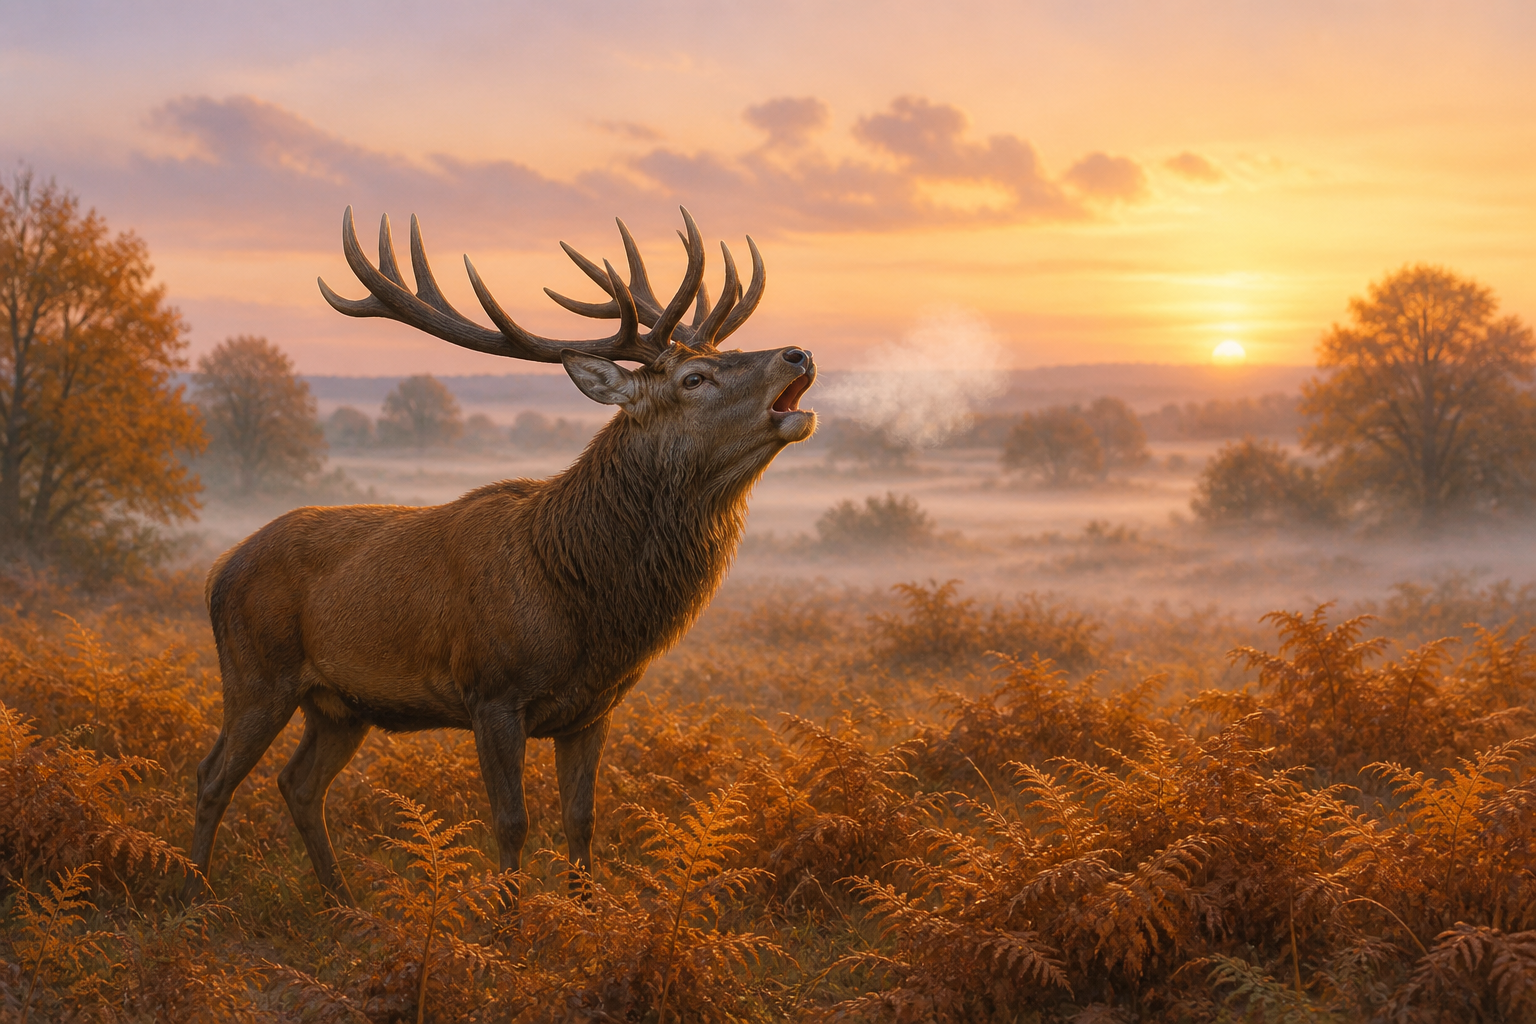
\includegraphics[width=0.6\linewidth]{images/book1/ai/g8-repro-stag.png}

{\small पतझड़ की गरज, वसंत का गणित: बारहसिंगे का समय गर्भ के महीने
गिनकर चलता है।}
\end{omfigure}

\begin{omfigure}
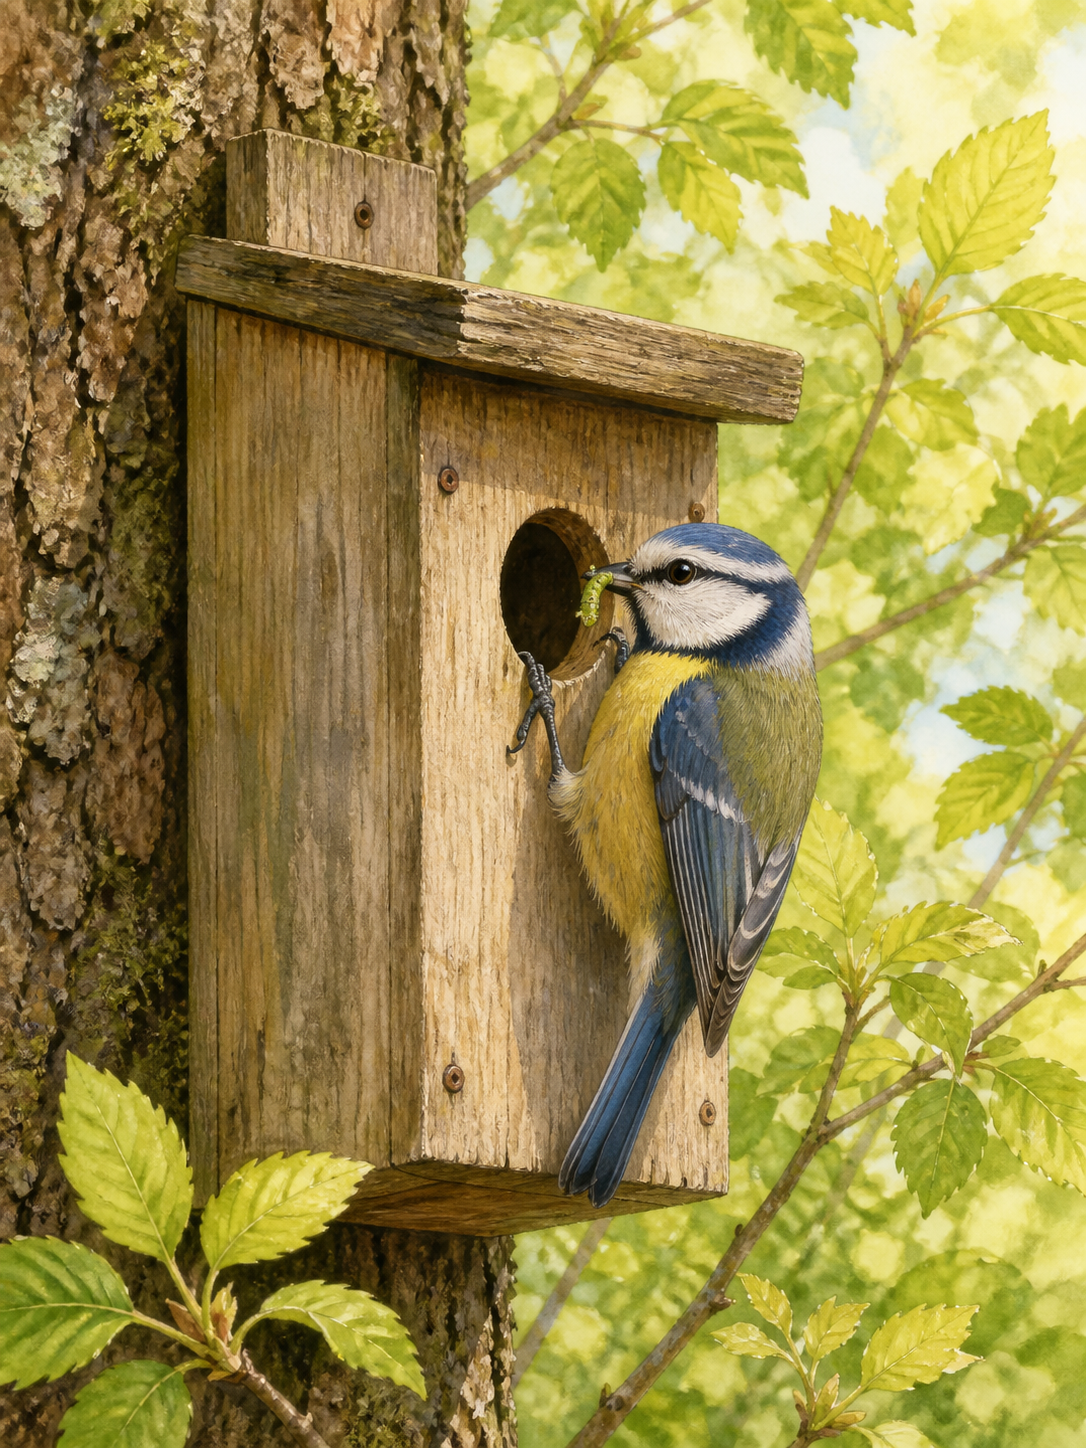
\includegraphics[width=0.46\linewidth]{images/book1/ai/g8-env-nestbox.png}

{\small \omterm{def:g2:where-animals-live:habitat}{आवास} की गुणवत्ता, घर तक पहुँचाई हुई: एक नीली चिड़िया, और वह
\omterm{ex:g2:animals-grow-up:butterfly}{इल्ली} जिस पर उसके \omterm{def:g2:animals-grow-up:born}{अंडों} का समय सधा था।}
\end{omfigure}

\begin{example}[भीतर पले मेमने]\label{ex:g8:reproduction-and-environment:lambs}
भेड़ पालने वाले इस संकेत का सीधे फ़ायदा उठाते हैं: भेड़ें तब प्रजनन की
हालत में आती हैं जब दिन \emph{छोटे} होने लगते हैं; और बनावटी तौर पर पहले
लंबे, फिर छोटे किए गए \omterm{def:g6:exploring-our-environment:conditions}{प्रकाश} में रखकर पूरे रेवड़ को उस वक़्त मेमने देने
लायक़ बनाया जा सकता है जब बाज़ार में सबसे ज़्यादा फ़ायदा हो। मशीनरी
\omterm{def:g6:exploring-our-environment:conditions}{प्रकाश} पढ़ती है, कैलेंडर नहीं --- \omterm{def:g6:exploring-our-environment:conditions}{प्रकाश} बदलो और कैलेंडर पीछे-पीछे चला
आता है। जो संकेत पहचान लिया जाए वह एक लीवर बन जाता है।
\end{example}

\section{आवास से मिला साज़-सामान}

\begin{proposition}[जनन का दाम पदार्थ में चुकाया जाता है]\label{prop:g8:reproduction-and-environment:cost}
\omterm{def:g2:animals-grow-up:born}{अंडे}, \omterm{def:g2:animals-grow-up:born}{दूध}, मकरंद, \omterm{def:g2:from-seed-to-plant:seed}{बीज} और सींग, सब
\cref{def:g6:matter-from-food:production} के अर्थ में
\emph{निर्माण} हैं --- यानी वह \omterm{def:g6:plants-are-producers:matter}{कार्बनिक पदार्थ}, जो जनकों को पहले
हासिल करना पड़ता है। इसलिए बजट \omterm{def:g2:where-animals-live:habitat}{आवास} की समृद्धि तय करती है:
\begin{itemize}
  \item भरपेट खाई मुर्ग़ी रोज़ \omterm{def:g2:animals-grow-up:born}{अंडा} देती है; भूखी रुक जाती है ---
        यानी \cref{pb:g6:matter-from-food:1} वाला बहीखाता, \omterm{def:g2:animals-grow-up:born}{अंडे} की
        पंक्ति पर मिलता हुआ;
  \item बीच का \omterm{def:g1:plants-around-us:tree}{पेड़} भारी \omterm{prop:g3:flowers-fruits-seeds:transform}{फल} सिर्फ़ ``बहुफल सालों'' में देता है, और वे
        भी अच्छे बढ़वार वाले मौसमों के बाद --- \omterm{def:g2:from-seed-to-plant:seed}{बीज} की \omterm{def:g6:producing-our-food:farming}{फ़सलें} बैंक में
        रखी हुई गर्मियाँ हैं
        (\cref{ex:g6:plants-are-producers:pantry});
  \item और कठिन साल \omterm{def:g2:animals-grow-up:born}{अंडों} की संख्या घटा देते हैं: शिकार कम हो तो
        बहुत-से \omterm{prop:g3:sorting-living-things:groups}{पक्षी} कम \omterm{def:g2:animals-grow-up:born}{अंडे} देते हैं, या देते ही नहीं।
\end{itemize}
\end{proposition}
\admitted

\begin{example}[चिड़िया के अंडे गिनना]\label{ex:g8:reproduction-and-environment:clutch}
घोंसला-डिब्बों के अध्ययन दिखाते हैं कि नीली चिड़िया के \omterm{def:g2:animals-grow-up:born}{अंडों} की संख्या
\omterm{ex:g2:animals-grow-up:butterfly}{इल्लियों} की आपूर्ति के पीछे-पीछे चलती है: बलूत के समृद्ध जंगलों में दस
या उससे ज़्यादा \omterm{def:g2:animals-grow-up:born}{अंडे}; ग़रीब बग़ीचों में छह या सात। चिड़िया यह फ़ैसला
किसी बहीखाते से नहीं करती --- \omterm{def:g2:where-animals-live:habitat}{आवास} के भोजन से बना उसके शरीर का हाल ही तय
करता है कि वह कितनों का साज़-सामान जुटा सकती है। \omterm{def:g2:animals-grow-up:born}{अंडों} की संख्या यानी
\omterm{def:g2:where-animals-live:habitat}{आवास} की गुणवत्ता, \omterm{def:g2:animals-grow-up:born}{अंडों} में लिखी हुई।
\end{example}

\section{दुनिया की बाँधी हुई हद: आबादियाँ}

\begin{definition}[आबादी]\label{def:g8:reproduction-and-environment:population}
\emph{आबादी}\index{आबादी} किसी एक \omterm{def:g5:biodiversity:species}{प्रजाति} के वे सारे व्यक्ति हैं जो एक
ही जगह रहते हैं --- तालाब के मेंढक, जंगल के बीच के \omterm{def:g1:plants-around-us:tree}{पेड़}। जनन उसमें
जोड़ता है; मौतें और कूच घटाते हैं; और छत \omterm{def:g6:exploring-our-environment:components}{पर्यावरण} तय करता है।
\end{definition}

\begin{proposition}[आबादियाँ फटकर बढ़ क्यों नहीं जातीं]\label{prop:g8:reproduction-and-environment:limits}
हर \omterm{def:g5:biodiversity:species}{प्रजाति} ज़रूरत से ज़्यादा पैदा करती है --- मेंढकों की हर जोड़ी के
हज़ारों \omterm{def:g2:animals-grow-up:born}{अंडे}, बीच के हर \omterm{def:g1:plants-around-us:tree}{पेड़} के हज़ारों \omterm{def:g2:from-seed-to-plant:seed}{बीज}
(\cref{prop:g4:animal-reproduction:strategies}) --- फिर भी तालाब
मेंढकों से ठोस नहीं भर जाते। यह फ़ालतू \omterm{def:g6:exploring-our-environment:components}{पर्यावरण} की रोकों के ख़िलाफ़
ख़र्च हो जाता है:
\begin{itemize}
  \item \emph{शिकार} --- \cref{ex:g4:animal-reproduction:pondcount}
        वाले बगुले और व्याध-पतंगे के डिंभ;
  \item \emph{भोजन और जगह} --- \omterm{ex:g2:animals-grow-up:butterfly}{इल्लियाँ}, घोंसलों के खोखल और जंगल के
        फ़र्श पर पड़ते \omterm{def:g6:exploring-our-environment:conditions}{प्रकाश} के टुकड़े, सब गिनती के ही हैं;
  \item \emph{\omterm{def:g6:exploring-our-environment:conditions}{परिस्थितियाँ}} --- फूलों पर देर से पड़ा पाला
        (\cref{exo:g3:flowers-fruits-seeds:9}), और \omterm{ex:g2:animals-grow-up:frog}{टैडपोलों} के
        सिकुड़ते तालाब पर सूखा।
\end{itemize}
औसतन, किसी टिके हुए \omterm{def:g2:where-animals-live:habitat}{आवास} में, हर जोड़ी बस अपनी जगह भर लेती है ---
यानी \cref{prop:g5:food-webs:balance} वाला संतुलन, जनकों की तरफ़ से देखा
हुआ।
\end{proposition}
\admitted

\begin{example}[तालाब पर दो वसंत]\label{ex:g8:reproduction-and-environment:twosprings}
पहला वसंत, नरम और गीला: पानी ऊँचा, \omterm{prop:g3:sorting-living-things:groups}{कीट} जल्दी आए --- हज़ारों \omterm{def:g2:animals-grow-up:born}{अंडे},
सैकड़ों मेंढक के बच्चे, और \omterm{def:g8:reproduction-and-environment:population}{आबादी} चढ़ती हुई। दूसरा वसंत, एक सूखा: तालाब
सिकुड़कर गड्ढा रह गया, \omterm{ex:g2:animals-grow-up:frog}{टैडपोल} भीड़ में, \omterm{def:g7:what-is-respiration:respiration}{ऑक्सीजन} गिरी हुई
(\cref{prop:g7:oxygen-in-the-water:drains}), और बगुले उस गाढ़े हुए
झुंड पर दावत उड़ाते हुए --- नतीजा, गिनती भर मेंढक के बच्चे। वही मेंढक,
वही कार्य-प्रणाली, और दो अलग फ़ैसले: हर पीढ़ी पर आख़िरी दस्तख़त
\omterm{def:g6:exploring-our-environment:components}{पर्यावरण} के होते हैं।
\end{example}

\begin{remark}[इंसान रोकें खिसका देते हैं]\label{rem:g8:reproduction-and-environment:humans}
जंगली जीवन पर इंसान के ज़्यादातर असर इन्हीं रोकों से होकर चलते हैं,
केंद्रीय कार्य-प्रणाली से नहीं: सुखाए गए तालाब और उखाड़ी गई बाड़ें
प्रजनन का \omterm{def:g2:where-animals-live:habitat}{आवास} हटा देती हैं
(\cref{prop:g2:where-animals-live:loss}); कीटनाशक \omterm{ex:g2:animals-grow-up:butterfly}{इल्लियों} का वह शिखर
ख़ाली कर देते हैं जिस पर चिड़ियों ने अपना समय साधा था; और बग़ीचे के
घोंसला-डिब्बे तथा \cref{ex:g5:biodiversity:storks} वाली फिर से बहाल गीली
चरागाहें छत वापस जोड़ देती हैं। किसी \omterm{def:g5:biodiversity:species}{प्रजाति} की हिफ़ाज़त का असल मतलब है
उस \omterm{def:g6:exploring-our-environment:components}{पर्यावरण} की हिफ़ाज़त, जिसमें उसका जनन जुड़ा हुआ है --- यानी संकेत,
बजट और रोकें, तीनों साथ।
\end{remark}

\begin{method}[आबादी के बदलाव की जाँच-पड़ताल]\label{met:g8:reproduction-and-environment:audit}
कोई \omterm{def:g8:reproduction-and-environment:population}{आबादी} चढ़े या गिरे, तो क्रम से जाँच-पड़ताल करो:
\begin{enumerate}
  \item \emph{समय}: क्या संकेत और संसाधन का शिखर अब भी एक साथ पड़े?
        (बहुत जल्दी आया वसंत चूज़ों को \omterm{ex:g2:animals-grow-up:butterfly}{इल्लियों} के बाद अकेला छोड़
        सकता है);
  \item \emph{बजट}: उस मौसम के \omterm{def:g2:where-animals-live:habitat}{आवास} ने जनकों को कितना साज़-सामान
        जुटाने दिया?
  \item \emph{रोकें}: इनमें से क्या बदला --- शिकारी, भोजन, जगह,
        \omterm{def:g6:exploring-our-environment:conditions}{परिस्थितियाँ}?
  \item \emph{\omterm{def:g2:where-animals-live:habitat}{आवास}}: क्या प्रजनन की ज़मीन ख़ुद बढ़ी या घटी?
\end{enumerate}
\end{method}

\section{अभ्यास}

\begin{exercise}[$\star$]\label{exo:g8:reproduction-and-environment:1}
नीली चिड़िया जब \omterm{def:g2:animals-grow-up:born}{अंडे} देती है तभी क्यों देती है? नियम बताओ, और संकेत भी।
\end{exercise}

\begin{exercise}[$\star$]\label{exo:g8:reproduction-and-environment:2}
बारहसिंगे का पतझड़ वाला समय क्या हासिल करता है, और उसमें क्या गिनना
पड़ता है?
\end{exercise}

\begin{exercise}[$\star$]\label{exo:g8:reproduction-and-environment:3}
जनन का दाम ``पदार्थ में चुकाया'' क्यों जाता है?
\cref{prop:g8:reproduction-and-environment:cost} में से तीन दाम बताओ।
\end{exercise}

\begin{exercise}[$\star$]\label{exo:g8:reproduction-and-environment:4}
\omterm{def:g8:reproduction-and-environment:population}{आबादी} क्या है? उसमें क्या जोड़ता है, क्या घटाता है, और छत कौन तय करता
है?
\end{exercise}

\begin{exercise}[$\star$]\label{exo:g8:reproduction-and-environment:5}
वे तीन रोकें बताओ जो मेंढकों का फ़ालतू ख़र्च कर देती हैं।
\end{exercise}

\begin{exercise}[$\star$]\label{exo:g8:reproduction-and-environment:6}
चिड़िया के दस \omterm{def:g2:animals-grow-up:born}{अंडे} बनाम छह \omterm{def:g2:animals-grow-up:born}{अंडे} किस बात की, और किसके बारे में, ख़बर
देते हैं?
\end{exercise}

\begin{exercise}[$\star\star$]\label{exo:g8:reproduction-and-environment:7}
भेड़ पालने वालों की \omterm{def:g6:exploring-our-environment:conditions}{प्रकाश} वाली तरकीब समझाओ, और यह भी कि वह संकेतों के
बारे में क्या साबित करती है।
\end{exercise}

\begin{exercise}[$\star\star$]\label{exo:g8:reproduction-and-environment:8}
\cref{ex:g8:reproduction-and-environment:twosprings} को
\cref{met:g8:reproduction-and-environment:audit} के चार सवालों के रूप
में फिर से सुनाओ, और वह भी दूसरे वसंत के लिए जवाब देकर।
\end{exercise}

\begin{exercise}[$\star\star$]\label{exo:g8:reproduction-and-environment:9}
गरमाती आबोहवा बलूत की \omterm{ex:g2:animals-grow-up:butterfly}{इल्लियाँ} दो हफ़्ते पहले ले आती है, पर चिड़ियों का
दिन-की-लंबाई वाला संकेत जस-का-तस है। इस बेमेल की और उसकी जाँच-पंक्ति
की भविष्यवाणी करो।
\end{exercise}

\begin{exercise}[$\star\star$]\label{exo:g8:reproduction-and-environment:10}
``कॉड मछली के लाखों बरबाद नहीं होते --- वे ख़र्च होते हैं।'' इस वाक्य
का बचाव \cref{prop:g8:reproduction-and-environment:limits} से करो।
\end{exercise}

\begin{exercise}[$\star\star$]\label{exo:g8:reproduction-and-environment:11}
इनमें से हर इंसानी काम कौन-सी रोक खिसकाता है: किसी दलदल का सुखाया
जाना; घोंसला-डिब्बे टाँगना; मई में बाग़ पर \omterm{ex:g2:animals-grow-up:butterfly}{इल्लियों} के ख़िलाफ़ छिड़काव;
किसी गीली चरागाह की \omterm{def:g7:organs-at-work:recovery}{बहाली}?
\end{exercise}

\begin{exercise}[$\star\star\star$]\label{exo:g8:reproduction-and-environment:12}
तीन अध्यायों को एक ही अनुच्छेद में जोड़ो: रणनीति की लकीर
(\cref{prop:g4:animal-reproduction:strategies}), पिरामिड के नुक़सान
(\cref{ex:g6:matter-from-food:pyramid}), और इस अध्याय की रोकें ---
और वह भी इसी एक हिसाब की तरह कि तालाब मेंढकों से ठोस क्यों नहीं भर
जाता।
\end{exercise}

\section{समस्या: घोंसला-डिब्बों की बही}

\begin{problem}[{सप्ताहांत समस्या --- नीली चिड़ियों के दस साल,
डिब्बा-दर-डिब्बा जाँचे हुए}]\label{pb:g8:reproduction-and-environment:1}
एक स्कूल दस साल तक बीस घोंसला-डिब्बों पर नज़र रखता है: \omterm{def:g2:animals-grow-up:born}{अंडे} देने की
तारीख़ें, \omterm{def:g2:animals-grow-up:born}{अंडों} की संख्या, और हर डिब्बे से उड़ने वाले चूज़े --- और साथ
में मौसम का लेखा तथा माली की डायरी भी।

\medskip\noindent\textbf{भाग I --- सामान्य साल पढ़ना।}
\begin{enumerate}
  \item साल 1--4: \omterm{def:g2:animals-grow-up:born}{अंडे} अप्रैल के आख़िर में, आठ से दस की संख्या में,
        और ज़्यादातर \omterm{def:g2:animals-grow-up:born}{अंडों} से उड़ने लायक़ चूज़े। वह संकेत बताओ जो
        अप्रैल का आख़िर तय करता है, और वह शिखर भी जिस पर यह समय सधा
        है।
  \item साल 2 की गरम, \omterm{ex:g2:animals-grow-up:butterfly}{इल्लियों} से भरी मई के बाद साल 3 में \omterm{def:g2:animals-grow-up:born}{अंडे} एक-दो
        ज़्यादा रहे --- जनकों की सर्दी अच्छी बीती थी। यह मेल किस
        प्रतिज्ञप्ति को दिखाता है?
  \item अच्छे सालों में भी लगभग पाँचवाँ हिस्सा \omterm{def:g2:animals-grow-up:born}{अंडे} कभी उड़ने लायक़
        नहीं होते।
        \cref{prop:g8:reproduction-and-environment:limits} में से वे
        रोकें गिनाओ जो शायद ज़िम्मेदार हैं।
  \item स्कूल \omterm{def:g2:animals-grow-up:born}{अंडों} के साथ-साथ मौसम और अहाते के काम का लेखा क्यों
        रखता है? (जवाब जाँच-पड़ताल के चारों सवालों से दो।)
\end{enumerate}

\medskip\noindent\textbf{भाग II --- अनोखे साल।}
\begin{enumerate}[resume]
  \item साल 5: एक अजीब गरम मार्च \omterm{ex:g2:animals-grow-up:butterfly}{इल्लियाँ} दो हफ़्ते पहले ले आया; पर
        \omterm{def:g2:animals-grow-up:born}{अंडे} देने की तारीख़ें मुश्किल से हिलीं। साल 5 में चूज़ों के
        उड़ने की भविष्यवाणी करो, और जाँच-पड़ताल की उस पंक्ति का नाम
        बताओ जो नाकाम हुई।
  \item साल 6: माली की डायरी में पुराने बलूतों की सूखी शाखाएँ हटाने
        और चरागाह की पट्टी हर महीने काटने का ज़िक्र है। मौसम मेहरबान
        रहने पर भी चूज़ों का उड़ना गिर जाता है। यह डायरी जाँच-पड़ताल
        की कौन-सी पंक्तियों पर उँगली रखती है?
  \item साल 7: बाज़ों की एक जोड़ी वहाँ बस जाती है। \omterm{def:g2:animals-grow-up:born}{अंडों} की संख्या
        जस-की-तस है, पर उड़ने वाले चूज़ों की गिनती गिर जाती है।
        कौन-सी रोक खिसकी, और \emph{\omterm{def:g2:animals-grow-up:born}{अंडों}} वाली पंक्ति उसके साथ क्यों
        नहीं खिसकी?
  \item साल 8: डिब्बे दोगुने होकर चालीस कर दिए गए; कुल उड़ने वाले
        चूज़े बढ़ जाते हैं, पर \emph{हर डिब्बे} की कामयाबी वहीं की
        वहीं रहती है। नए डिब्बों ने कौन-सी छत ऊपर उठाई, और किसे उन्होंने
        छुआ तक नहीं?
\end{enumerate}

\medskip\noindent\textbf{भाग III --- रिपोर्ट।}
\begin{enumerate}[resume]
  \item दस साल का वह सार-वाक्य लिखो जो \omterm{def:g2:animals-grow-up:born}{अंडों} की संख्या को \omterm{def:g2:where-animals-live:habitat}{आवास} की
        गुणवत्ता से जोड़े, और
        \cref{ex:g8:reproduction-and-environment:clutch} का हवाला दे।
  \item नगर पालिका बलूतों की क़तार काटकर वहाँ गाड़ी खड़ी करने की जगह
        बनाने का प्रस्ताव रखती है, और उसकी ``भरपाई'' पचास और
        घोंसला-डिब्बों से करने की। इस पेशकश की जाँच करो: संकेत, बजट,
        रोकों और \omterm{def:g2:where-animals-live:habitat}{आवास} में से डिब्बे किसकी जगह लेते हैं, और कौन-सी
        चीज़ सिर्फ़ बलूत ही देते हैं?
  \item साल 11 के लिए अहाते के दो उपाय सुझाओ, और हर एक को उसकी
        जाँच-पंक्ति से बाँधो।
  \item अध्याय की सीख एक वाक्य में देकर बात ख़त्म करो: दो जनकों के
        अलावा हर उड़ने वाले चूज़े को और क्या चाहिए?
\end{enumerate}
\end{problem}
